

\begin{figure}[h]
\centering
    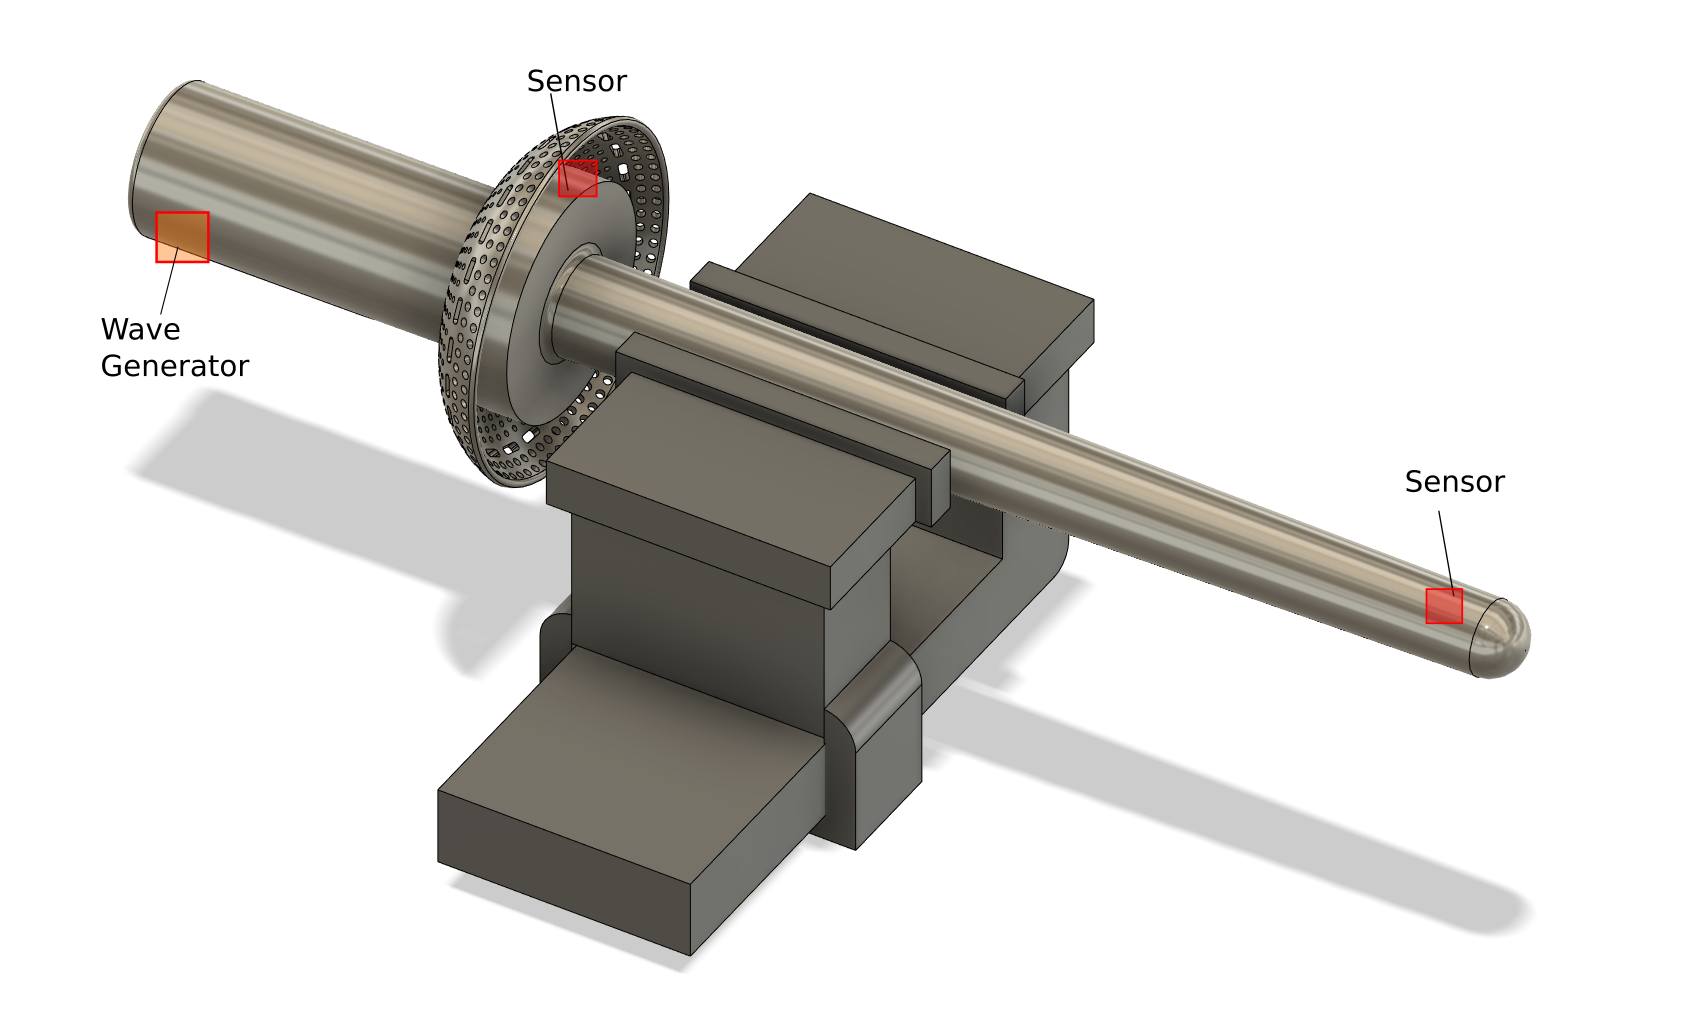
\includegraphics[width=\textwidth]{figures/experimental-setup.png}
\caption{}
\label{fig:}
\end{figure}

\subsection{ITAP dimensions}
\begin{table}[h]
    \centering
    \begin{tabular}{cc}
        \textbf{Stem} & Dimension \\ \hline
        diameter & 12 mm \\
        length & 120 mm \\
        &\\
        \textbf{Collar} & Dimensions\\ \hline
        height & 6 mm \\
        diameter & 28 mm \\
        & \\
        \textbf{Spigot} & Dimensions\\ \hline
        diameter & 18 mm \\
        length & 45 mm
    \end{tabular}
    \caption{Probably replace with technical drawing + description in prose}
    \label{tb:}
\end{table}
% Dimensions extracted from Kirstin's thesis

% Cemented for > 15mm and/or implant fixed above the isthmus of the diaphysis. Stem diameter such that there is 2mm of cement.
% Taper of 0.75 degrees.
% Radial cement grooves 1.5mm.

% IM < 15 mm, press fit. Anti rotation teeth (1 mm height) on distal third of their stems and an HA coating (150 to 200 um thick)

% fixed with four 6 mm grub screws

% \begin{table}[h]
% \centering
% \begin{tabular}{ccc }
%     \textbf{Stem} & Dimension & Notes \\ \hline
%     diameter & 9-15 mm & 12 narrowing to 9mm\\
%     length & 100-145 mm \\
%     & &\\
%     \textbf{Flange} & Dimensions & Notes \\ \hline
%     diameter & 24-35 mm \\
%     & &\\
%     \textbf{Spigot} & Dimensions& Notes\\ \hline
%     diameter & 18 mm & \\
%     length & ?? & \\
% \end{tabular}
% \caption{Dimensions extracted from K. Ahmed}
% \label{tb:}
% \end{table}

% \subsection{Frequencies}
% Clinically relevant frequencies, resonance, 

% Do modal analysis to find resonant frequencies. 

% We find resonant frequency, clinically we want to be below 
% - effect due to fulcrum, and some sort of symmetry around it
% Separate graphically

% independent variables: axis of displacement (x,y,z), frequency, displacement
% dependent: Magnitude displacement, x,y,z magnitude
% frequency less than resonance mode (approx 900)

% Points of interest: side of flange and tip. soft tissue adjacent to the collar will experience the force on the side of the collar

% Show a couple of examples

% Graph showing input displacement and the displacement at the points of interest


\subsection{Motivation for how this is being tackled}

\paragraph{Replication of physical model}

\paragraph{Assumptions and short-comings}


\paragraph{Sensor positioning}
Figure \ref{fig:10-300-900-max-displacements} shows the large variety of motion the model undergoes, hence the sensors at each position.

Link to reality in application: the displacement experienced on the soft tissue attached to the flange is likely the same as that experienced on the collar.

\begin{figure}[h] \centering
    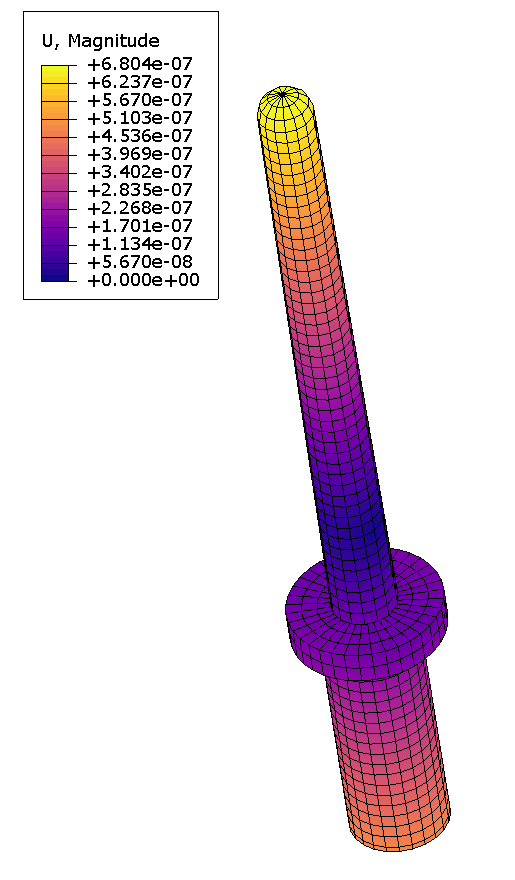
\includegraphics[width = 0.30\textwidth]{figures/Free/10hz.PNG}
    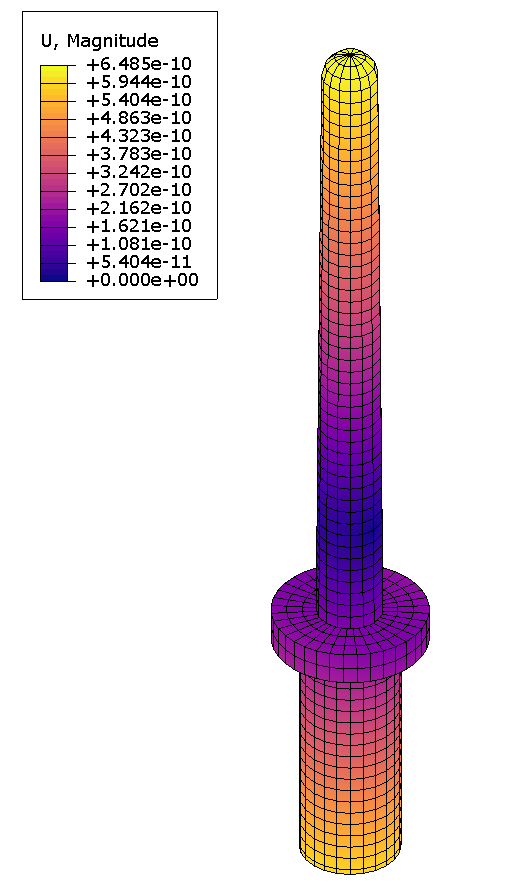
\includegraphics[width = 0.30\textwidth]{figures/Free/300hz.PNG}
    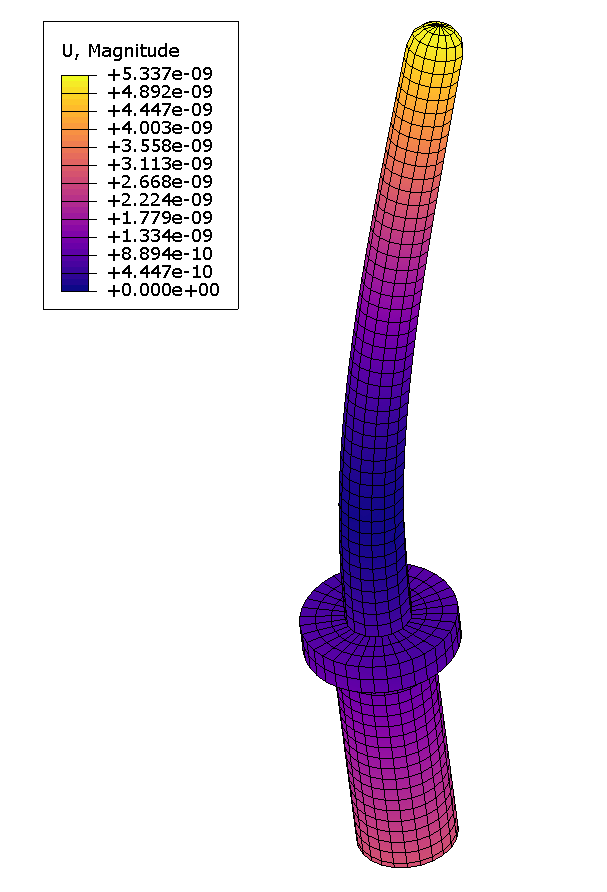
\includegraphics[width = 0.30\textwidth]{figures/Free/900hz.PNG}
\caption{Magnitude of displacement observed for 10hz, 300hz, 900hz, respectively. Intended to highlight why we place sensors on spigot, collar and stem. Not displayed is the scaling of the deflection}
\label{fig:10-300-900-max-displacements}
\end{figure}

\subsection{Modal analysis}
We know the range we want to operate, and we want to make sure there are no resonant frequencies within them.
So we do an analysis for the first ten modal frequencies.
Most importantly, the lowest is at 934 Hz, so we limit our simulations to between 1 Hz and 900 Hz.
Figure \ref{fig:modal-frequencies} shows what some of modes look like in simulation
\begin{figure}[h] \centering
    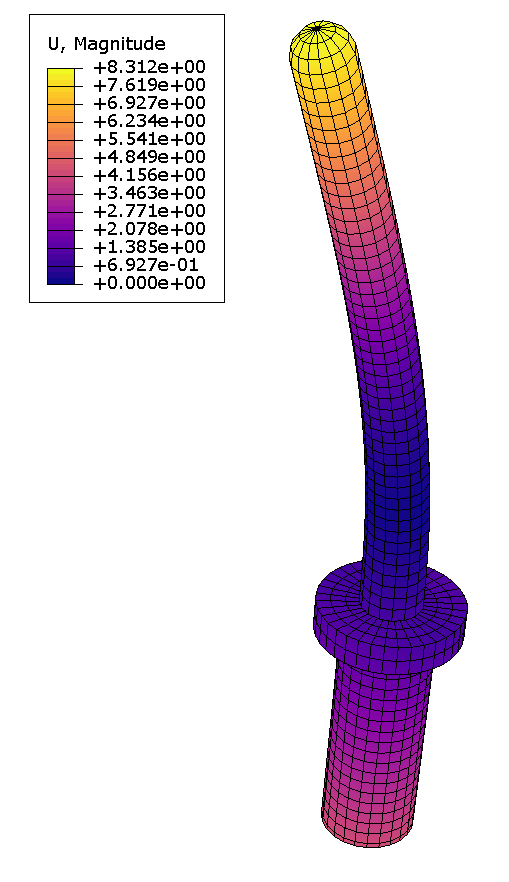
\includegraphics[width = 0.45\textwidth]{figures/934.png}
    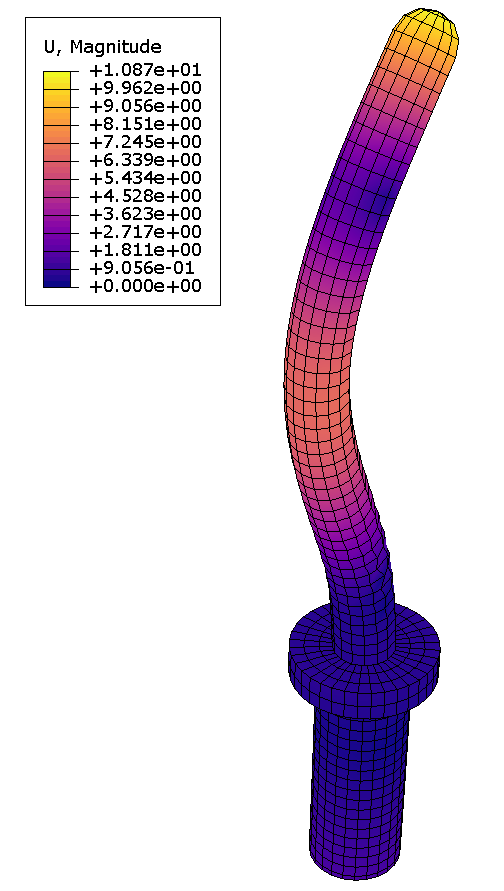
\includegraphics[width = 0.45\textwidth]{figures/3933.PNG}
\caption{Some of the modal frequencies observed for our model. Depicted are 934 Hz (left) and 3933 Hz (right). This informs the decision of keeping frequencies below the first mode.}
\label{fig:modal-frequencies}
\end{figure}